\documentclass[tikz]{standalone}
\usepackage{tikz}
\usetikzlibrary{positioning, shapes, fit, backgrounds, calc, arrows.meta}

% Declare the layers
\pgfdeclarelayer{background}
\pgfdeclarelayer{docker}
\pgfsetlayers{background,docker,main}

\begin{document}
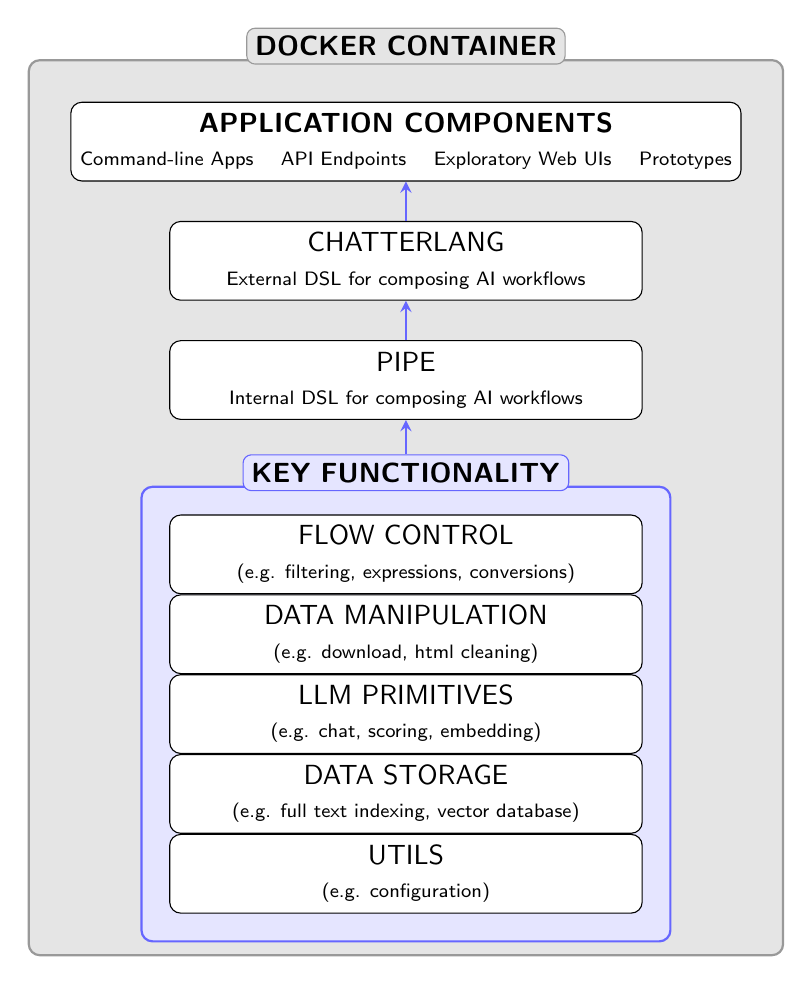
\begin{tikzpicture}[
  box/.style={rectangle, draw, rounded corners, minimum width=6cm, minimum height=1cm, align=center, fill=white},
  keylayer/.style={draw=blue!60, fill=blue!10, thick, rounded corners, inner sep=10pt},
  dockerlayer/.style={draw=gray!80, fill=gray!20, thick, rounded corners, inner sep=15pt},
  arrow/.style={->, thick, blue!60, >=stealth},
  font=\sffamily
]
% Key Functionality nodes
\node[box] (flow)                             {FLOW CONTROL\\\scriptsize (e.g. filtering, expressions, conversions)};
\node[box, below=0cm of flow] (data)          {DATA MANIPULATION\\\scriptsize (e.g. download, html cleaning)};
\node[box, below=0cm of data] (llm)           {LLM PRIMITIVES\\\scriptsize (e.g. chat, scoring, embedding)};
\node[box, below=0cm of llm] (store)          {DATA STORAGE\\\scriptsize (e.g. full text indexing, vector database)};
\node[box, below=0cm of store] (utils)        {UTILS\\\scriptsize (e.g. configuration)};

% Pipe - increased spacing to accommodate label
\node[box, above=1.2cm of flow] (pipe)        {PIPE\\\scriptsize Internal DSL for composing AI workflows};

% ChatterLang
\node[box, above=0.5cm of pipe] (chatter)     {CHATTERLANG\\\scriptsize External DSL for composing AI workflows};

% Application Layer
\node[box, above=0.5cm of chatter] (app) {
  \textbf{APPLICATION COMPONENTS}\\
  \scriptsize Command-line Apps \quad API Endpoints \quad Exploratory Web UIs \quad Prototypes
};

% Docker container background around all (bottom layer)
\begin{pgfonlayer}{background}
  \node[dockerlayer, fit=(app)(utils)] (docker-bg) {};
\end{pgfonlayer}

% Key Functionality background box (middle layer)
\begin{pgfonlayer}{docker}
  \node[keylayer, fit=(flow)(data)(llm)(store)(utils)] (key-bg) {};
\end{pgfonlayer}

% Key Functionality label (main layer - centered at top)
\node[at=(key-bg.north), anchor=south, yshift=-2pt, fill=blue!10, inner sep=3pt, draw=blue!60, rounded corners=3pt] (kfbox) {\textbf{KEY FUNCTIONALITY}};

% Docker label (main layer - centered at top)
\node[at=(docker-bg.north), anchor=south, yshift=-2pt, fill=gray!20, inner sep=3pt, draw=gray!80, rounded corners=3pt] {\textbf{DOCKER CONTAINER}};

% Arrows connecting the components
\draw[arrow] (kfbox.north) -- (pipe.south);
\draw[arrow] (pipe.north) -- (chatter.south);
\draw[arrow] (chatter.north) -- (app.south);

\end{tikzpicture}
\end{document}
